\documentclass{beamer}
\usetheme{Copenhagen}
\usecolortheme{whale}

\usepackage{graphicx}
%\usepackage{animate}
\usepackage{multimedia}
\usepackage{fontawesome}

\title{Efficient machine learning for causal effects}
\logo{
\includegraphics[scale=0.25]{../images/unc_sph.png}}
\author{Paul Zivich}
\institute{University of North Carolina at Chapel Hill}
\date{\today}
\setbeamercovered{transparent}
\setbeamertemplate{navigation symbols}{}
\setbeamertemplate{headline}{}

\AtBeginSection[]{
	\begin{frame}
		\vfill
		\centering
		\begin{beamercolorbox}[sep=8pt,center,shadow=true,rounded=true]{title}
			\usebeamerfont{title}\insertsectionhead\par%
		\end{beamercolorbox}
		\vfill
	\end{frame}
}

\begin{document}

\begin{frame}[plain]
    \maketitle
\end{frame}

\begin{frame}{Outline}
	\begin{enumerate}
		\item Motivating problem
		\item Identification
		\begin{itemize}
			\item Assumptions
		\end{itemize}
		\item Estimation
		\begin{itemize}
			\item High-dimensional data
			\item Solutions to the problem
			\item Model misspecification
			\item Machine learning
			\item Cross-fitting
		\end{itemize}
		\item Simulations
		\item Implementation
		\item Conclusion
	\end{enumerate}
\end{frame}

\begin{frame}{Quick Note on Efficiency}
	Efficiency refers to \textit{statistical} efficiency of an estimator
	\begin{itemize}
		\item Low mean squared error
	\end{itemize}~\\
	Cross-fitting procedures are not \textit{computationally} efficient
\end{frame}

\begin{frame}{Notation}
	$Y_i$: observed outcome of interest for individual $i$\\~\\
	$X_i$: observed exposure or treatment of interest\\~\\
	$Y_i(x)$: potential outcome under exposure set to $x$\\~\\
	$Z_i$: covariate(s)\\~\\
\end{frame}

\begin{frame}{Motivating Problem}
	Our collaborators want us to help them address what the difference in the risk of atherosclerotic cardiovascular disease ($Y$) had been if everyone was given statins ($x=1$) compared to if no one was given statins ($x=0$)? 
	\[\psi = E[Y(x=1)] - E[Y(x=0)]\]
	They are planning on collecting some observational (non-investigator randomized) data to address this.
\end{frame}

\section{Identification}

\begin{frame}{Identifiability Assumptions}
	Need to determine under what assumptions the average causal effect is \textit{identifiable}\\~\\
	One set of identifiability assumptions
	\begin{itemize}
		\item Causal consistency
		\item Conditional exchangeability
		\item Positivity
	\end{itemize}~\\
\end{frame}

\begin{frame}{Causal Consistency}
	An assumption regarding the potential outcomes observed
	\begin{itemize}
		\item We are able to observe at least one for some individuals
	\end{itemize}~\\
	For $X$ can write as
	$$Y_i = Y_i(x) \text{ if } x=X_i$$
	or as the treatment-variation irrelevance analog
	$$Y_i = Y_i(x, b) \text{ for all } b \in B$$
	where $b$ could be versions of statins (e.g., 10mg vs 100mg)
\end{frame}

%\begin{frame}{Causal Consistency}
%	An alternative way to think about this assumption
%	\begin{itemize}
%		\item 	Consider the general potential outcome
%		$$Y_i(x, x_{-i}, b)$$
%		where $x_{-i}$ is $x$ for all units besides $i$
%		\item 	Under the assumption of no interference, $x_{-i}$ is not necessary
%		$$Y_i(x, b)$$
%		\item Under the assumption of treatment-variation irrelevance
%		$$Y_i(x)$$
%	\end{itemize}
%\end{frame}

\begin{frame}{Conditional Exchangeability}
	Synonyms
	\begin{itemize}
		\item No unmeasured confounding
		\item Potential outcomes of ASCVD are conditionally independent of statin use
		\item No unmeasured common causes of statins and ASCVD
	\end{itemize}~\\
	Requires substantive knowledge outside of the data
	\begin{itemize}
		\item Directed Acyclic Graph
		\item Single-World Intervention Graph
	\end{itemize}
\end{frame}

%\begin{frame}{Directed Acyclic Graph}
%	\centering
%	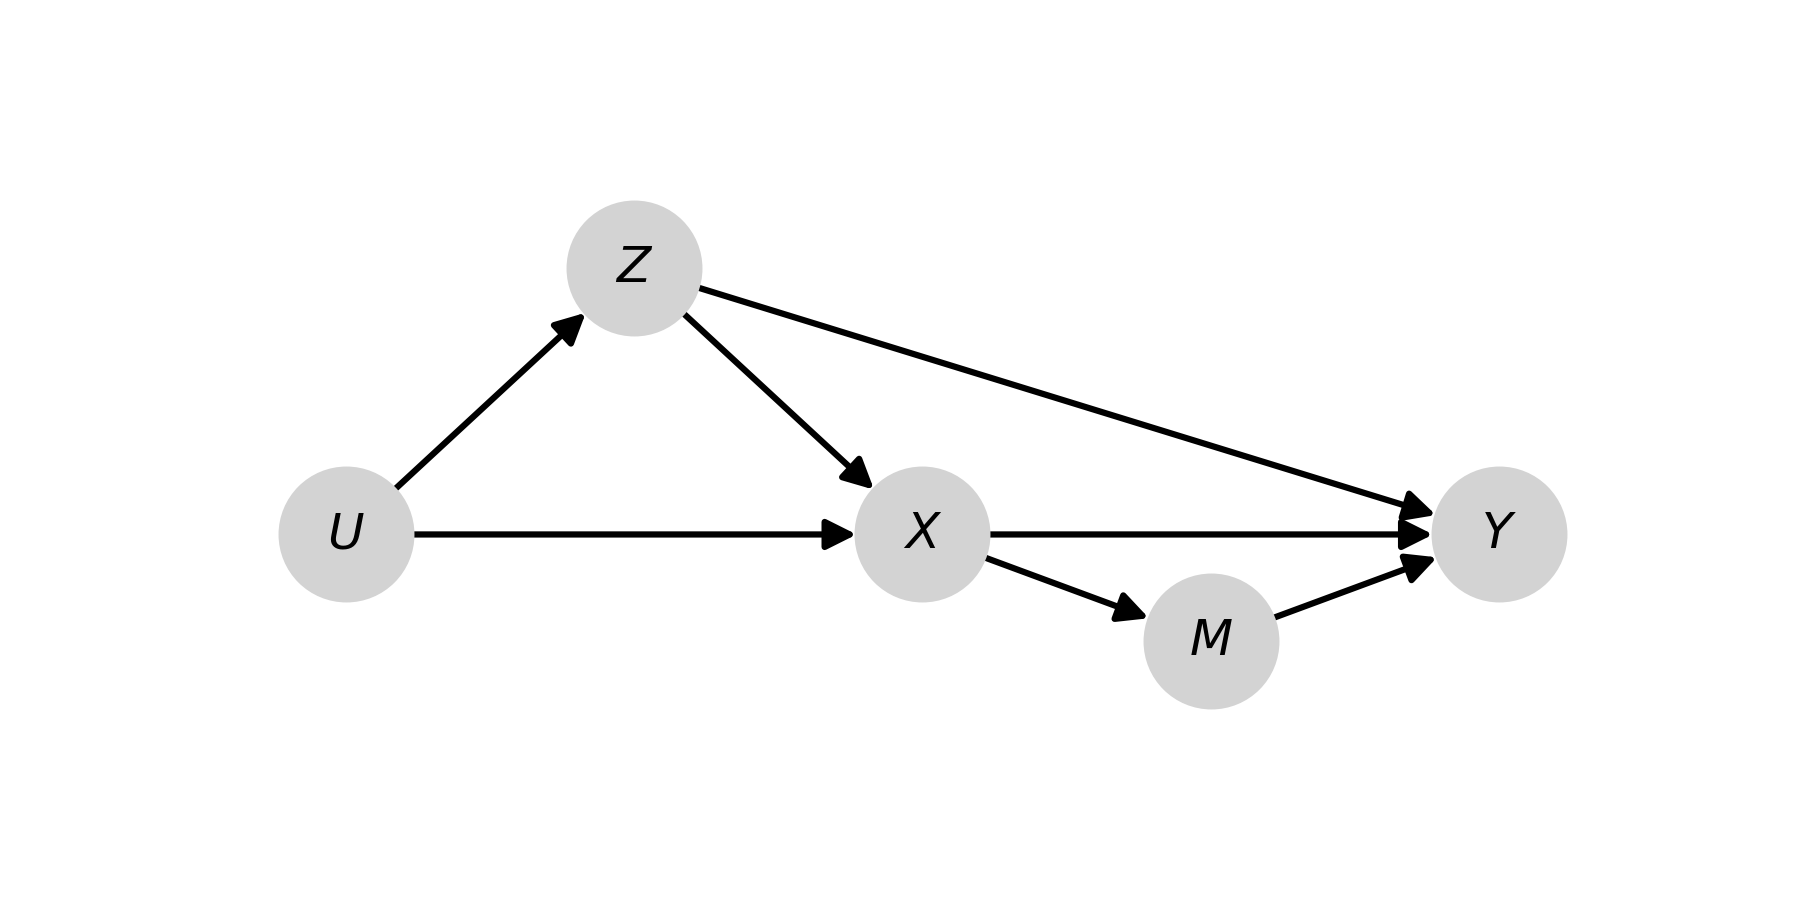
\includegraphics[scale=0.75]{images/dag.png}
%\end{frame}

\begin{frame}{Positivity}
	Conditional exchangeability requires that the probability for all values of statins to be non-zero in all strata of the confounders	
	\[\text{if } \Pr(Z=z)>0 \text{ then } \Pr(X=x|Z=z)>0\]~\\
	Positivity violations
	\begin{itemize}
		\item Some individuals never have access to statins
		\item Example: statins for children under 18 without inherited hypercholesterolemia 
	\end{itemize}
\end{frame}

\section{Estimation}

\begin{frame}{Motivating Problem}
	After discussion with our collaborators, the following covariates are determined to be confounders:
	\begin{itemize}
		\item Age
		\item Low-density lipoprotein (LDL)
		\item American Heart Association's ASCVD risk scores
		\item Diabetes
	\end{itemize} 
\end{frame}

\begin{frame}{Model-free Causal Inference}
	When $Z$ is low-dimensional
	\begin{itemize}
		\item No model is required
		\item Directly apply the non-parametric g-formula
		\item Unlikely in practice
	\end{itemize}~\\
	Our $Z$ includes continuous covariates (LDL, ASCVD risk scores)
	\begin{itemize}
		\item Model-free is not an option
	\end{itemize}
\end{frame}

\begin{frame}{High-Dimensional Data}
	High-dimensional data 
	\begin{itemize}
		\item Continuous $Z$ or more strata of $z$ than $n$
		\begin{itemize}
			\item LDL can range from less than 100 to more than 190
		\end{itemize}
		\item Sparse data in comparison to data dimension
	\end{itemize}~\\
	How can we make progress?
	\begin{itemize}
		\item Categorize
		\begin{itemize}
			\item E.g., LDL as $<$140, 140-159, 160-189, 190+
		\end{itemize}
		\item Model
	\end{itemize}
\end{frame}

\begin{frame}{Categorize}
	% \animategraphics[loop,controls,width=\linewidth]{10}{images/cat_gif/i}{0}{49}
	\centering
	\movie[width=4in,height=2.55in,poster,showcontrols]{.}{categorization.mov}
\end{frame}


\begin{frame}{Model}
	Model is an \textit{a priori} restriction on the distribution of the data
	\begin{itemize}
		\item Parametric model restricts to a parametric distribution
		\item Not necessary for identification
		\item Adds information not in the data
	\end{itemize}~\\
	Two processes can choose to model (nuisance models)
	\begin{itemize}
		\item exposure-model: $\Pr(X|Z;\alpha) = \pi(Z;\alpha)$
		\item outcome-model: $\Pr(Y|X=x,Z;\beta) = m_x(Z;\beta)$
	\end{itemize}
\end{frame}

\begin{frame}{No Model Misspecification}
	Addition of information via a model is not free
	\begin{itemize}
		\item Requires the addition of assumption on model specification
		\item True density is within model's ($\mathcal{M}$) class of densities 
		\item exposure-model: $\Pr(X|Z) \in \mathcal{M}_{\alpha}$
		\item outcome-model: $\Pr(Y|X,Z) \in \mathcal{M}_{\beta}$
	\end{itemize}~\\
	Implications
	\begin{itemize}
		\item Suggests use of flexible models
	\end{itemize}
\end{frame}

\begin{frame}{Doubly Robust Estimators}
	Clever combination of $\pi(Z;\alpha)$ and $m_x(Z;\beta)$
	\begin{itemize}
		\item Consistent as long as one model is correct
		\item Two chances for parametric model
	\end{itemize}~\\
	Common doubly-robust estimators
	\begin{itemize}
		\item Augmented inverse probability weighting
		\item Targeted maximum likelihood estimation
	\end{itemize}
\end{frame}

%\begin{frame}{Augmented Inverse Probability Weighting (AIPW)}
%	\[\hat{\psi}_{AIPW}(x) = n^{-1} \sum_i \frac{I(X_i=x) Y_i}{\widehat{\pi}(Z_i)} + \frac{\widehat{m_x}(Z_i) (\widehat{\pi}(Z_i) - I(X_i=x))}{\widehat{\pi}(Z_i)}\]~\\
%	\begin{itemize}
%		\item Improved efficiency compared to IPW estimator
%		\begin{itemize}
%			\item Double-robustness is a 'free' side-effect
%		\end{itemize}
%	\end{itemize}~\\
%	\[\hat{\psi}_{AIPW}(x) = n^{-1} \sum_i \widehat{m_x}(Z_i) + \frac{(Y_i - \widehat{m_x}(Z_i)) I(X_i=x)}{\widehat{\pi}(Z_i)}\]
%	\begin{itemize}
%		\item Double-robustness compared to g-computation
%		\begin{itemize}
%			\item Price: loss of efficiency
%		\end{itemize}
%	\end{itemize}
%\end{frame}

\begin{frame}{Machine Learning}
	Data-adaptive estimators (machine learning)
	\begin{itemize}
		\item Less restrictive than parametric modeling
		\begin{itemize}
			\item Capture wider class of densities
		\end{itemize}
		\item May be more reasonable to believe flexible enough model
		\begin{itemize}
			\item Or that model is sufficiently close
		\end{itemize}
	\end{itemize}
\end{frame}

\begin{frame}{Machine Learning}
	\large
	Problems in Application
	\begin{enumerate}
		\item Convergence
		\item Complexity
	\end{enumerate}
\end{frame}

\begin{frame}{Convergence}
	Remainder term goes to zero as function of $n$
	\begin{itemize}
		\item \textit{Not} computational complexity issue
		\begin{itemize}
			\item \textbf{NOT} when software says 'did not converge'
			\item Inherent feature of the estimators
		\end{itemize}
		\item How fast standard error of estimators decreases with $n$
		\item For inference, root-n ($n^{-1/2}$) is desirable
		\begin{itemize}
			\item Parametric models meet this criteria
			\item Data-adaptive likely don't
		\end{itemize}
		\item Slower than $n^{-1/2}$ may result in invalid inference
		\begin{itemize}
			\item Estimated variance is too small
			\item Implies greater certainty than true
		\end{itemize}
	\end{itemize}
\end{frame}

\begin{frame}{Convergence}
	\centering
	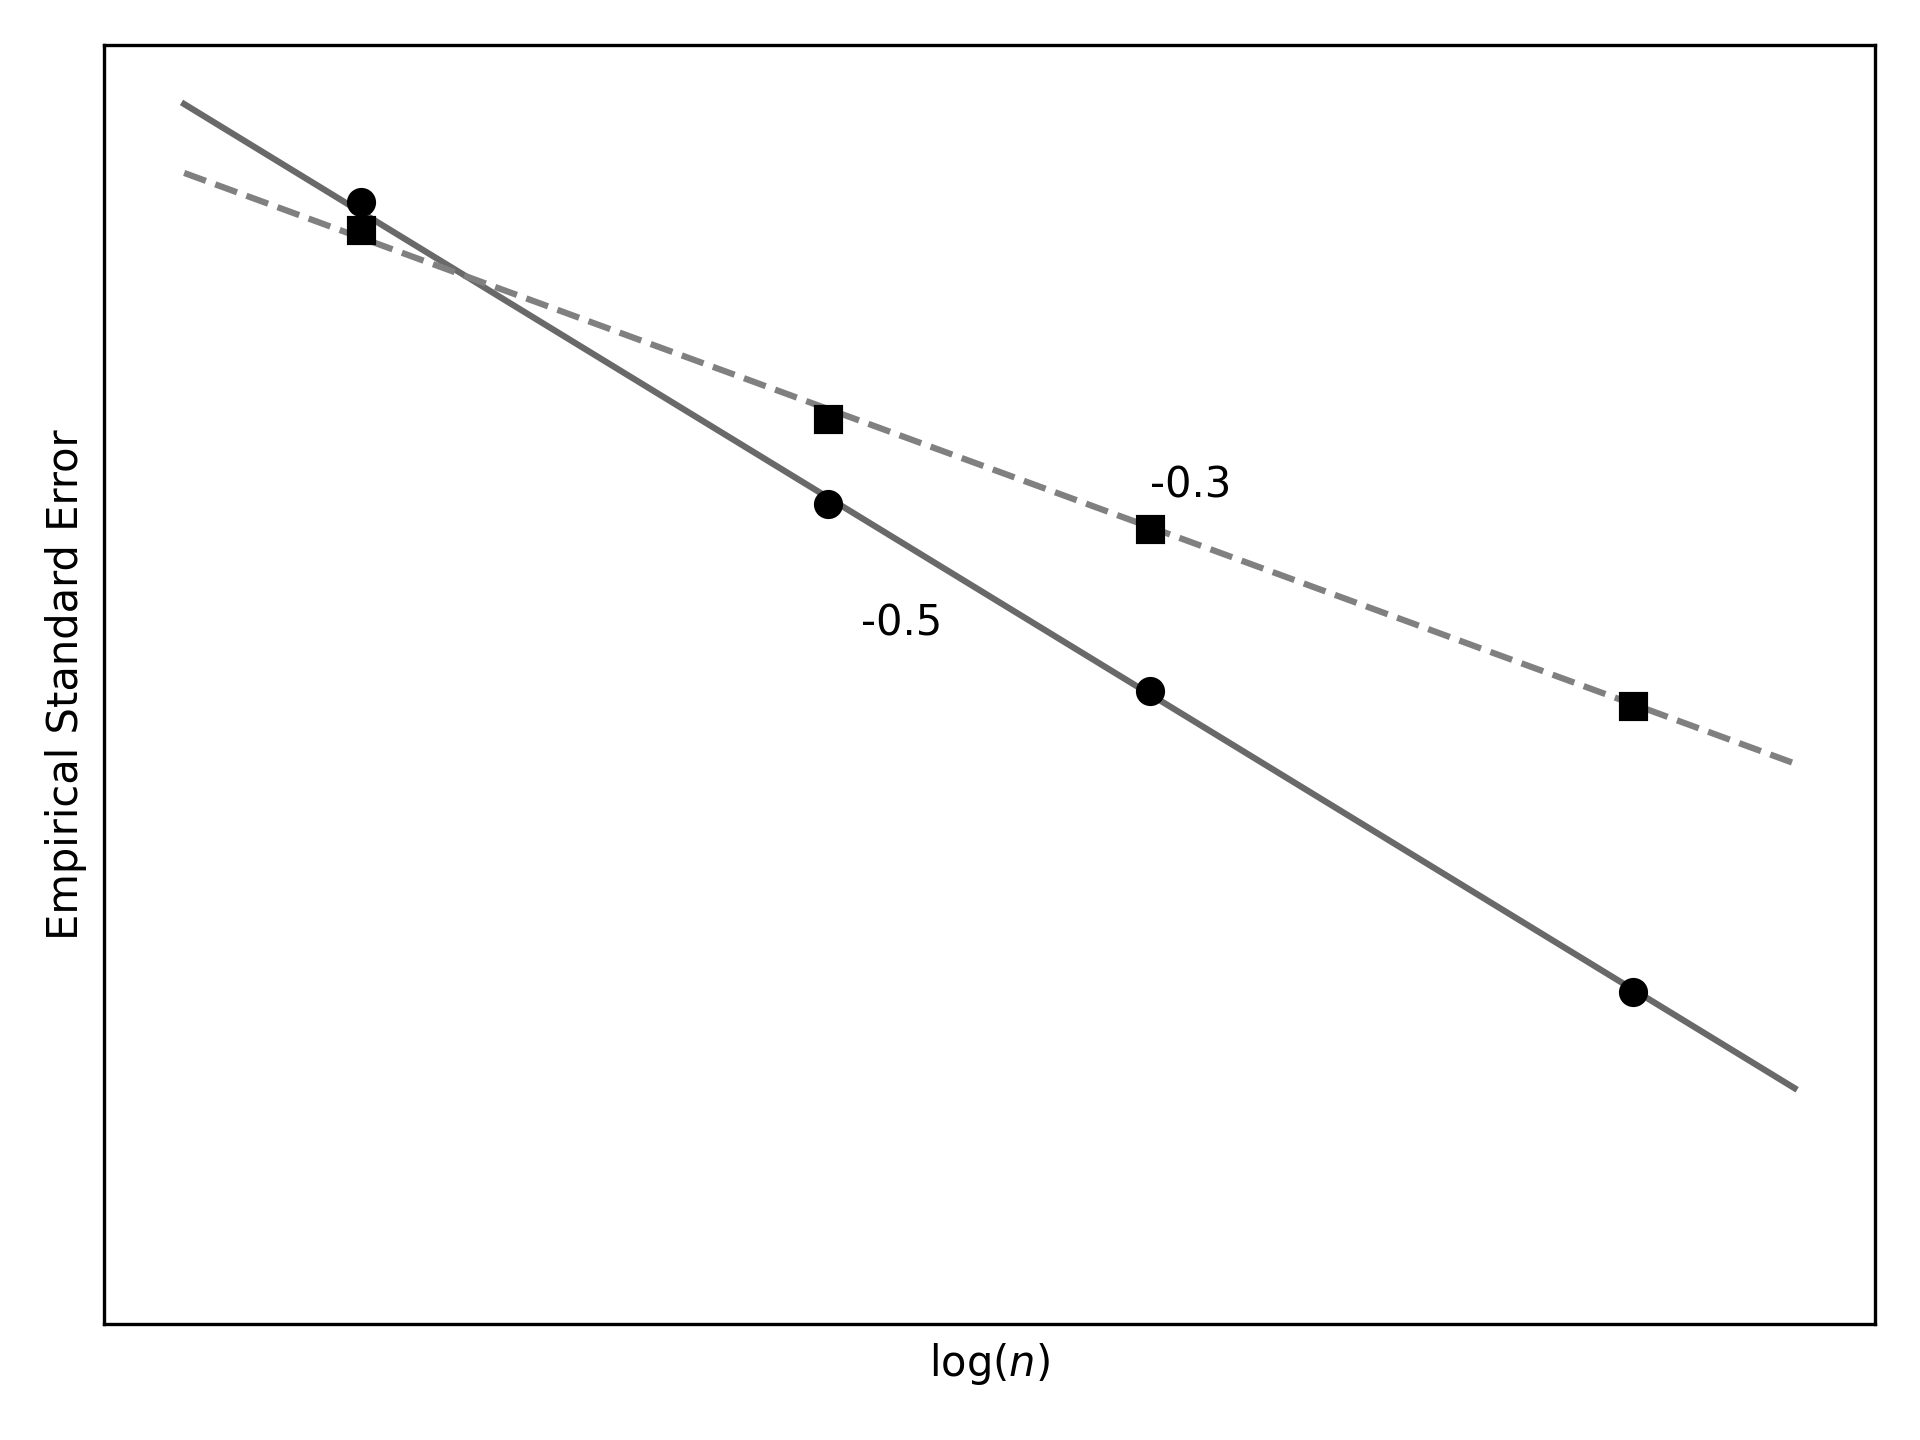
\includegraphics[scale=0.54]{images/convergence.png}
\end{frame}

\begin{frame}{Convergence and AIPW}
	AIPW can allow for slower convergence
	\begin{itemize}
		\item Under the assumption that both models are correct
		\begin{itemize}
			\item Second-order bias is a product of the approximation errors
			\item Only need at least $n^{-1/4}$ for both models 
		\end{itemize}~\\
		\item Wider range of models can be validly used with AIPW
		\begin{itemize}
			\item Comes at cost of double-robustness
			\item Becomes more akin to \textbf{\textit{double-susceptible}}
			\item Maybe okay if we use flexible models?
		\end{itemize}
	\end{itemize}
\end{frame}

\begin{frame}{Complexity}
	Restrictions on the complexity of a model
	\begin{itemize}
		\item Allows borrowing of information across observations
		\item Restricted to Donsker class
	\end{itemize}~\\
	Why restricting to Donsker is inappropriate
	\begin{itemize}
		%\item Robins' CODA Asymptotic Theory
		%\begin{itemize}
		%	\item Does not correspond to practice with moderate $n$
		%\end{itemize}
		\item Machine learning
		\begin{itemize}
			\item Dimension allowed to increase with $n$
			\item Exist in highly complex spaces
		\end{itemize}
	\end{itemize}
\end{frame}

\begin{frame}{Cross-fitting}
	Approach to relax Donsker class restriction
	\begin{itemize}
		\item Estimate model in one split and predict in other split
		\item Since from different sample
		\begin{itemize}
			\item Avoid the Donsker class restriction
		\end{itemize}
	\end{itemize}~\\
	Synonyms
	\begin{itemize}
		\item Sample splitting 
		\item Double machine learning
		\item Cross-validated
	\end{itemize}
\end{frame}

\begin{frame}{Single Cross-fit}
	\centering
	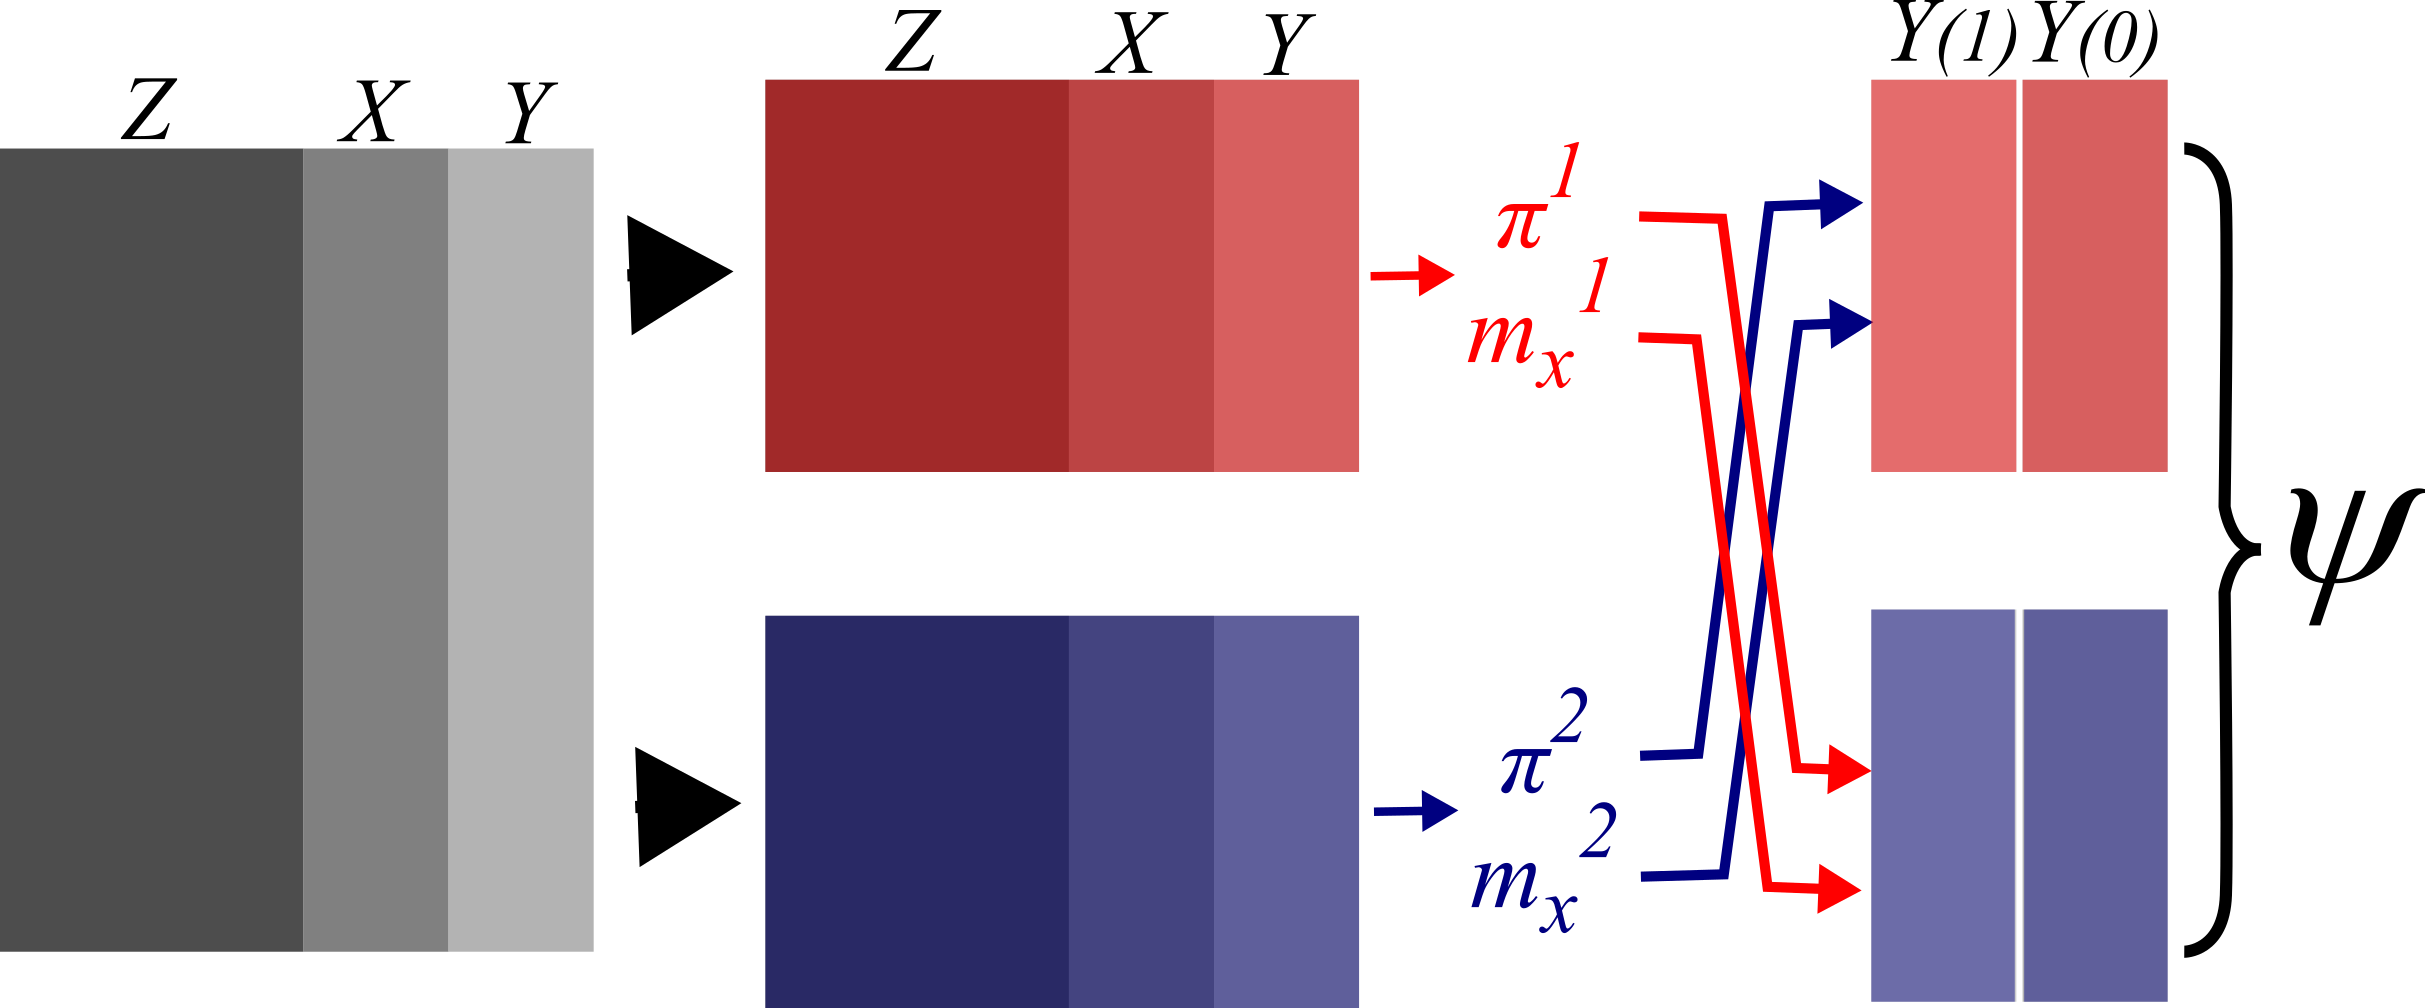
\includegraphics[scale=0.54]{images/single_xfit.png}
\end{frame}

\begin{frame}{Single Cross-fit}
	Removes own-observation bias
	\begin{itemize}
		\item Best data-adaptive estimator memorizes the data
		\begin{itemize}
			\item Highly predictive for the data
			\item Poor out-of-sample performance
		\end{itemize}
		\item Cross-fit prevents correlation between estimator and data
		\begin{itemize}
			\item Without need for Donsker class
		\end{itemize}
	\end{itemize}
\end{frame}

\begin{frame}{Double Cross-fit}
	\centering
	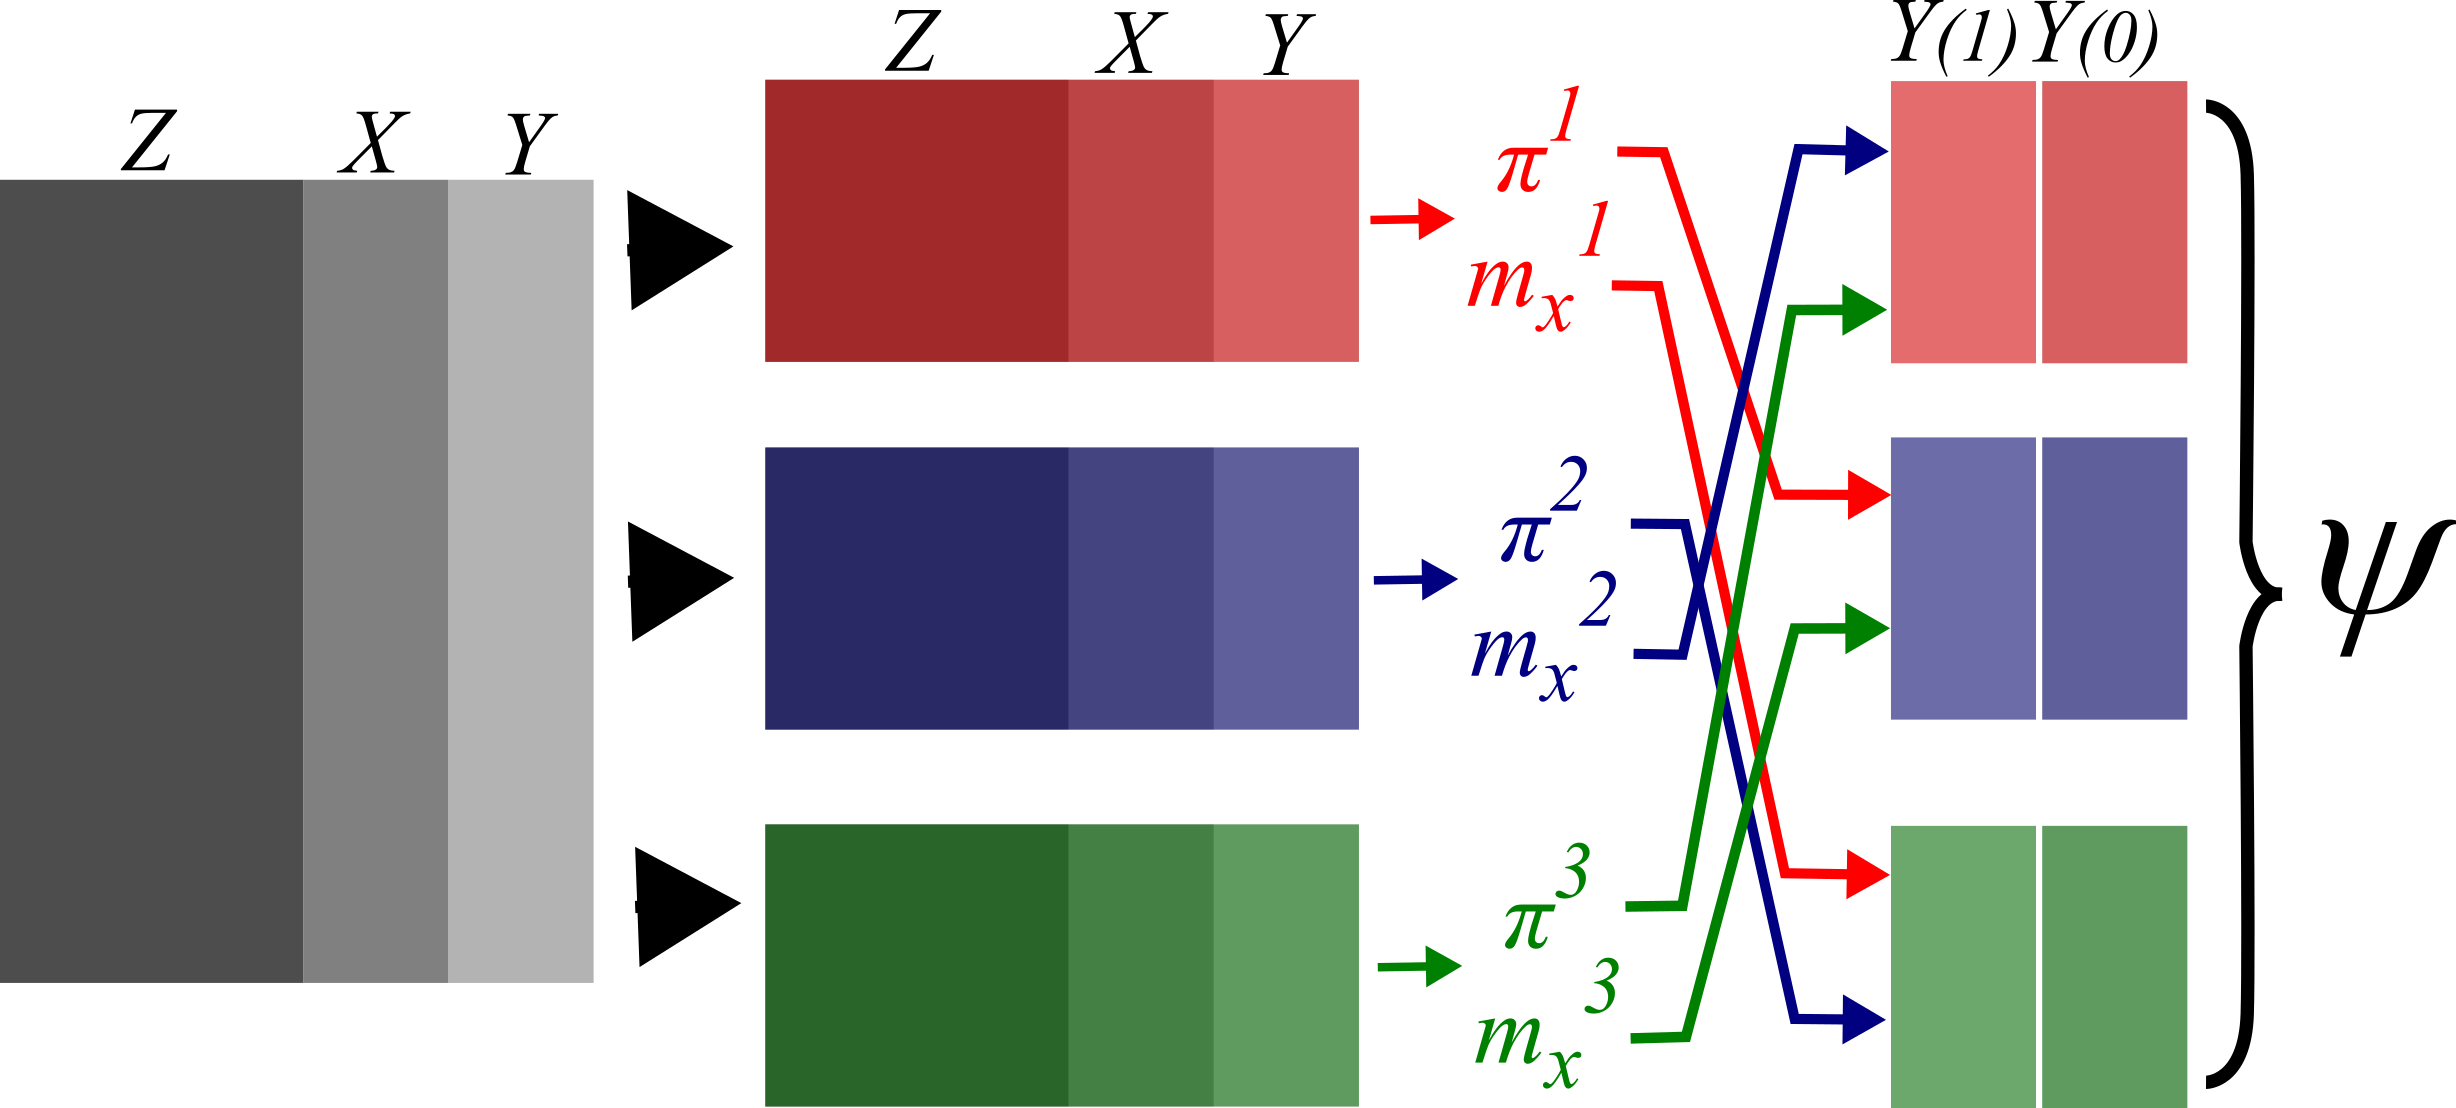
\includegraphics[scale=0.54]{images/double_xfit.png}
\end{frame}

\begin{frame}{Double Cross-fit}
	Removes own-observation bias \& non-linearity
	\begin{itemize}
		\item Cross-fit prevents correlation between estimator and data
		\begin{itemize}
			\item Without need for Donsker class
		\end{itemize}~\\
		\item Further de-couples data and estimators
		\begin{itemize}
			\item Compared to single cross-fit
		\end{itemize}
	\end{itemize}
\end{frame}

\begin{frame}{Looking Back...}
	\centering
	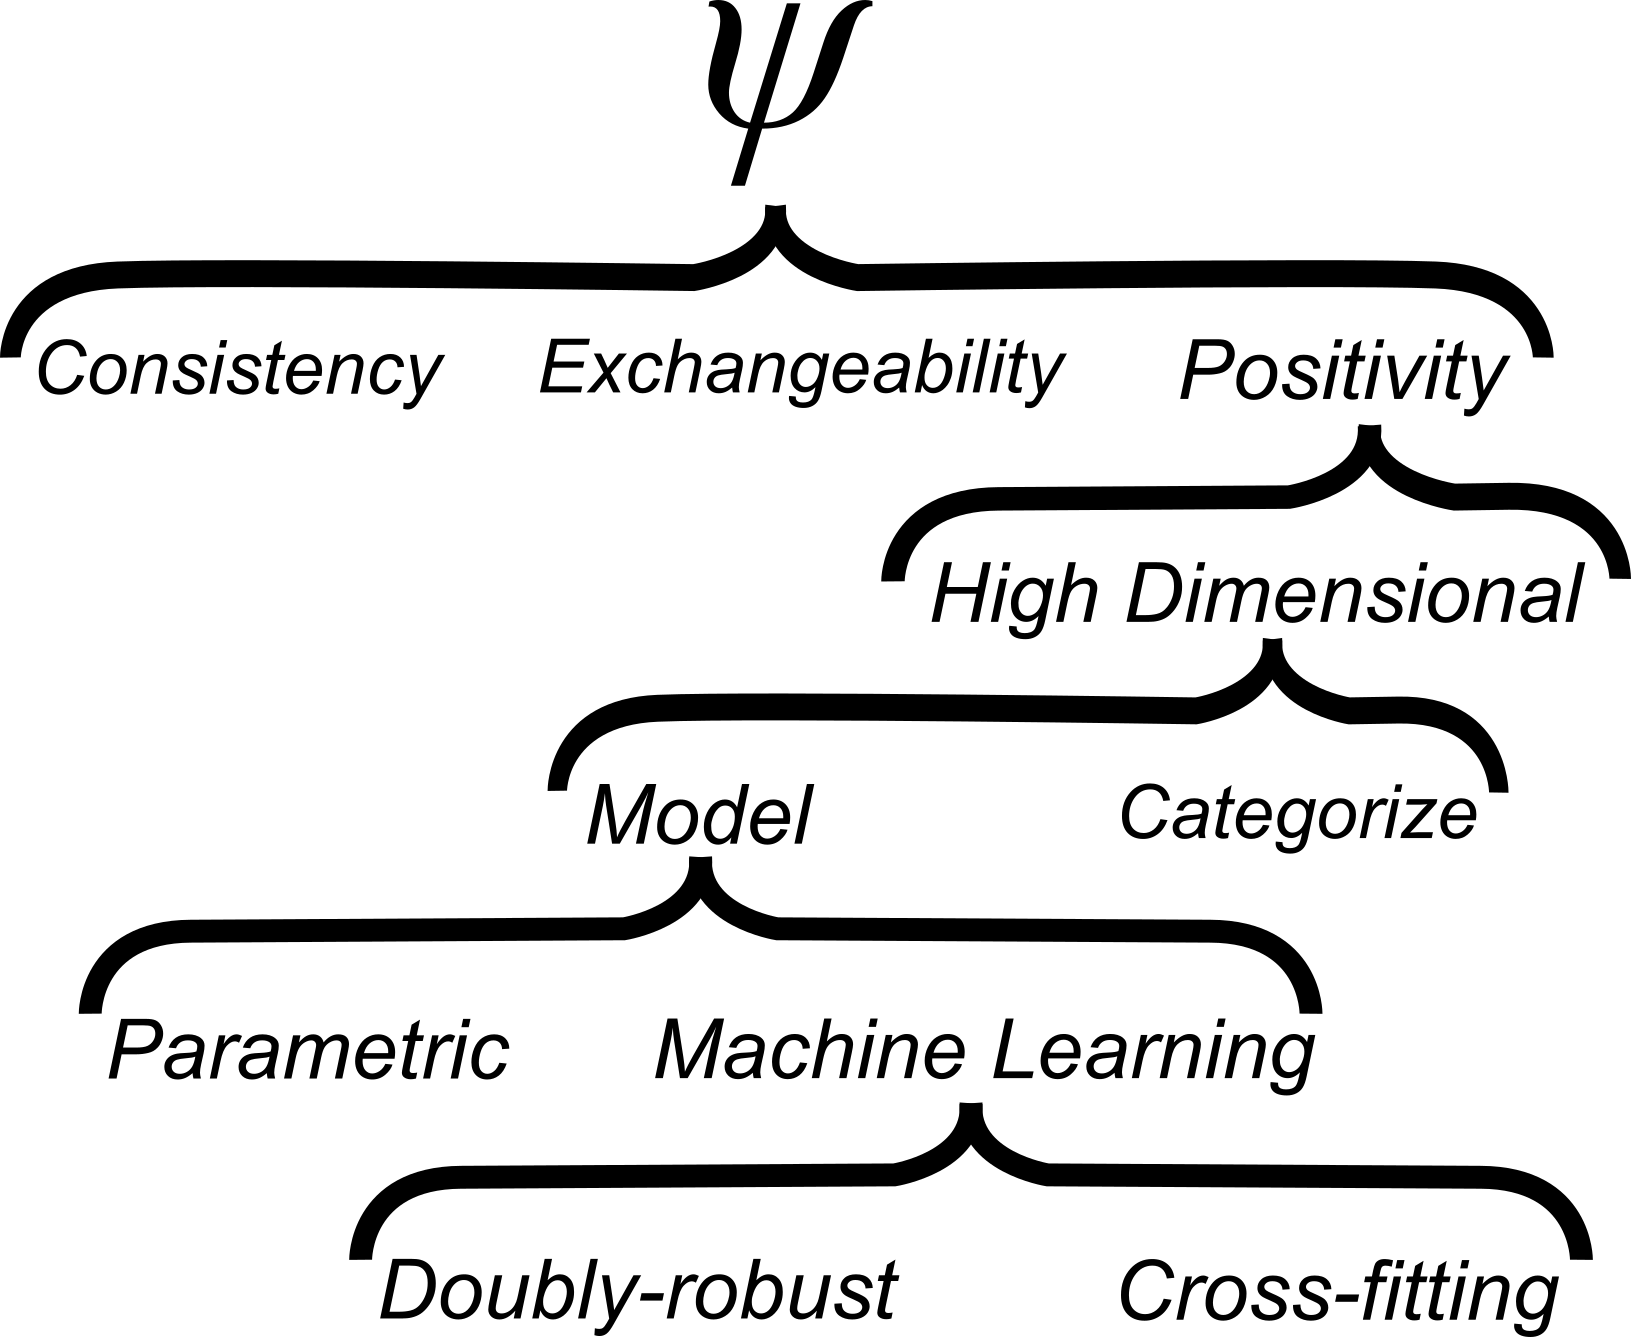
\includegraphics[scale=0.54]{images/tree_travel.png}
\end{frame}

\section{Simulations}

\begin{frame}{Data Generation}
	Average Causal Effect of Statins on ASCVD
	\begin{itemize}
		\item Age, low-density lipoprotein, ASCVD risk scores, diabetes
		\item 2000 reps with $n=3000$
	\end{itemize}~\\
	Metrics
	\begin{itemize}
		\item Bias
		\item 95\% Confidence interval coverage
	\end{itemize}
\end{frame}

\begin{frame}{Approaches}
	ACE estimators
	\begin{itemize}
		\item AIPW
		\item TMLE
		\item Double Cross-fit (DC-)AIPW
		\item DC-TMLE
	\end{itemize}~\\
	Nuisance model estimators
	\begin{itemize}
		\item Correct parametric model
		\item Main-effect parametric model
		\item Machine learning
	\end{itemize}
\end{frame}

% TODO super learner

\begin{frame}{Simulation Results}
	\centering
	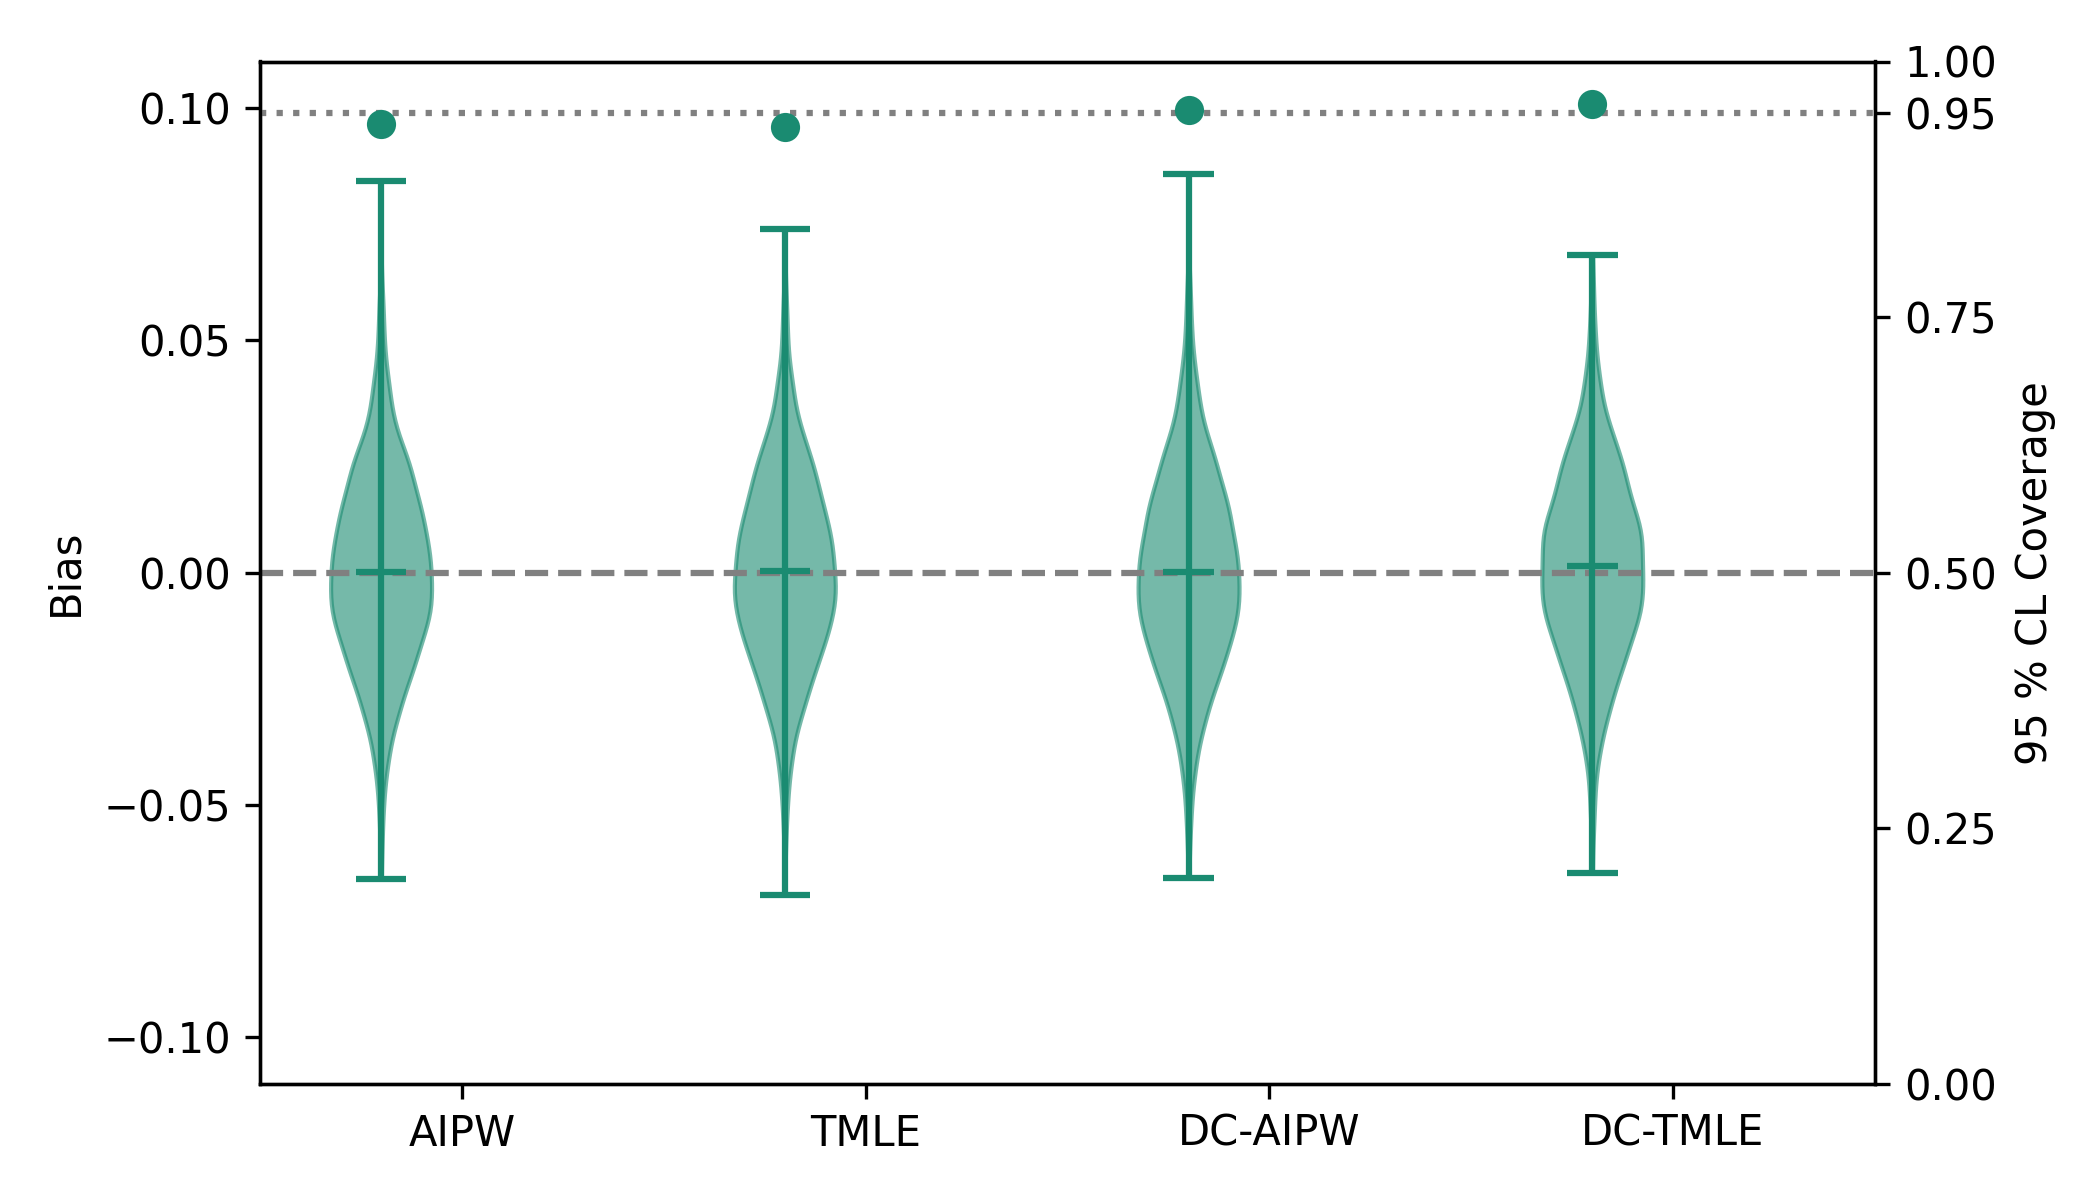
\includegraphics[scale=0.62]{images/sim_result1.png}
\end{frame}

\begin{frame}{Simulation Results}
	\centering
	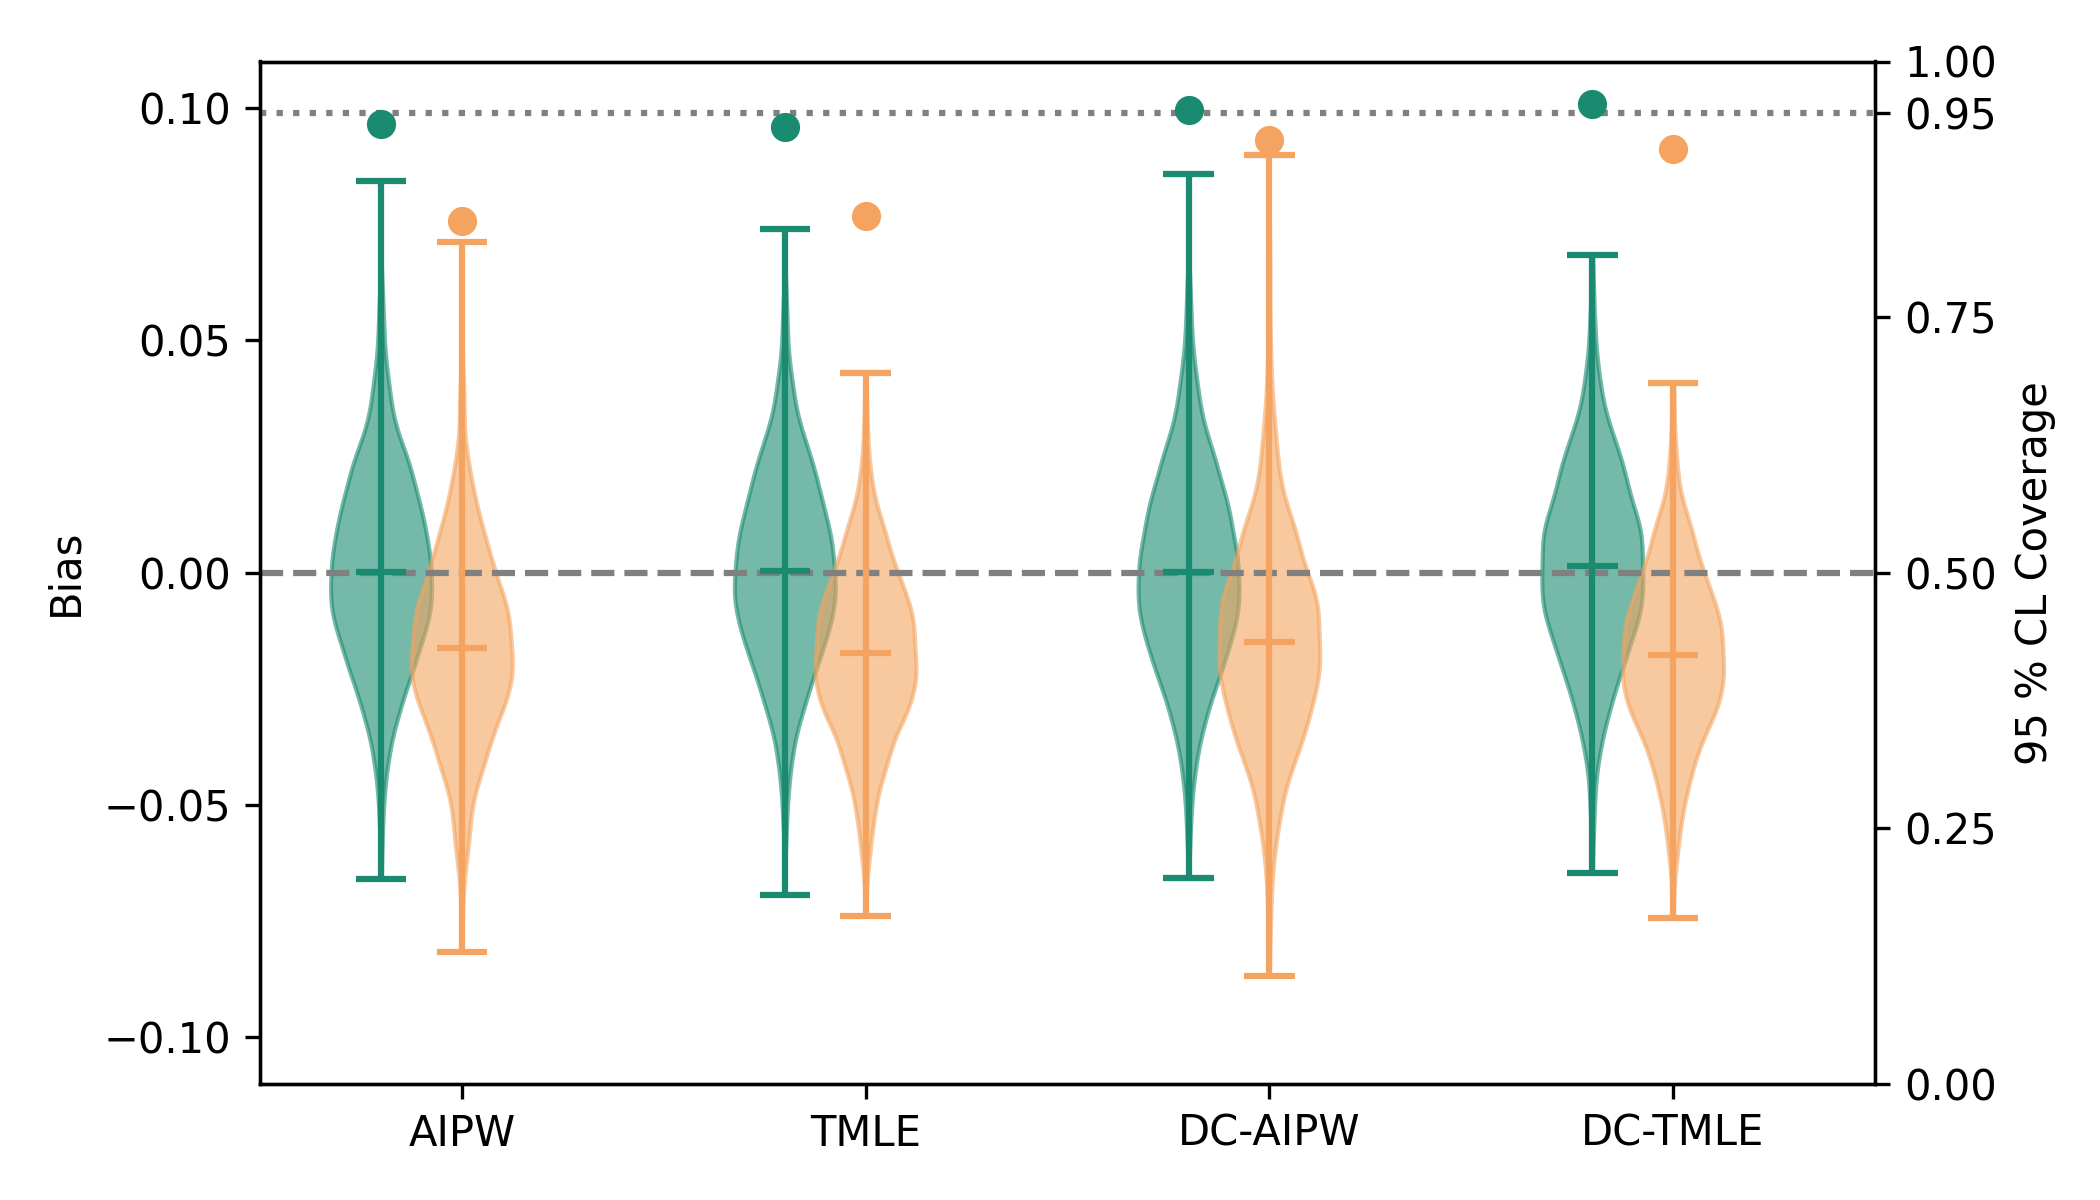
\includegraphics[scale=0.62]{images/sim_result2.png}
\end{frame}

\begin{frame}{Simulation Results}
	\centering
	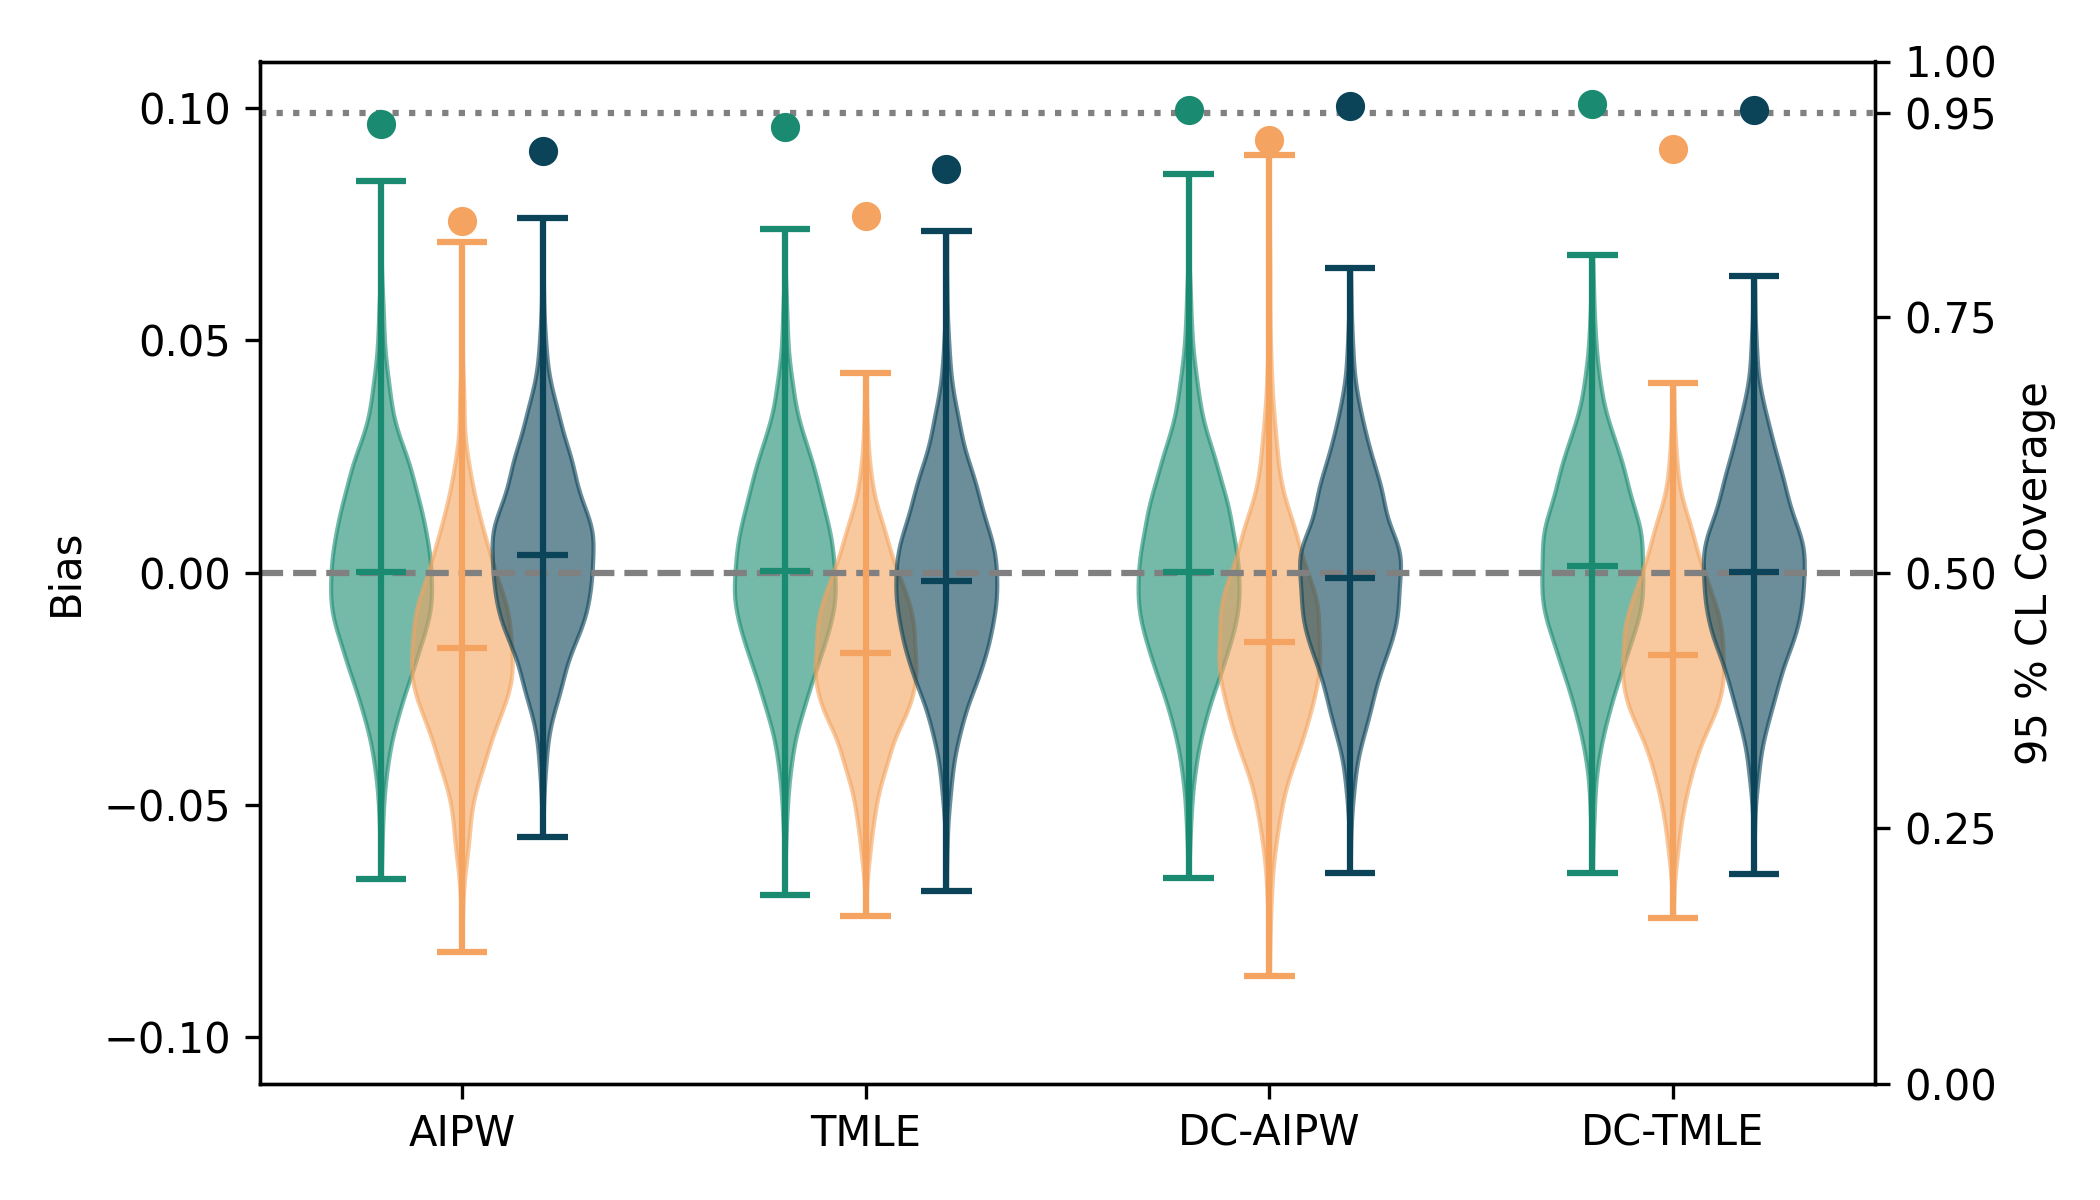
\includegraphics[scale=0.62]{images/sim_result3.png}
\end{frame}

\section{Implementation}

\begin{frame}{Partition versus Split}
	Split
	\begin{itemize}
		\item Observations grouped into non-overlapping, equal-sized groups
		\item Let $s$ indicate the number of splits for a data set
		\begin{itemize}
			\item $s=2$ randomly splits observations into two groups
		\end{itemize}
	\end{itemize}~\\
	Partition
	\begin{itemize}
		\item A particular division of splits
		\item E.g., IDs 1,2,4 are in split 1 and IDs 3,5,6 are in split 2		
	\end{itemize}
\end{frame}

\begin{frame}{Algorithm Pseudo-Code}
	Repeat for $p$ different partitions
	\begin{enumerate}
		\item Partition data into $s$ non-overlapping splits
		\item For each $s$:
		\begin{itemize}
			\item Estimate $\hat{\pi}^s(Z_i^s)$
			\item Estimate $\hat{m}_x^s(Z_i^s)$
		\end{itemize}
		\item For each $s$:
		\begin{itemize}
			\item Predict $\hat{\pi}^{\bar{s}} (Z_i^s)$
			\item Predict $\hat{m}_x^{\bar{s}}(Z_i^s)$
			\item Generate $\hat{Y}_i^*$
			\item Estimate $\psi^s$
			\item Estimate $Var(\psi^s)$
		\end{itemize}
		\item Estimate $\psi^p$ as mean of $\hat{\psi}^s$
		\item Estimate $Var(\psi^p)$ as mean of $\widehat{Var}(\hat{\psi}^s)$
	\end{enumerate}
	Summarize all partitions with~\\ 
	$\;\;\;\; \hat{\psi} = \text{median}(\hat{\psi}^p)\text{;} \;\;\;\;\;\;\; \widehat{Var}(\hat{\psi})$
\end{frame}

\begin{frame}{Step 1: Partition Data into Splits}
	\centering
	
\includegraphics[scale=0.7]{images/step1_split.png}
\end{frame}

\begin{frame}{Step 2: Estimate Nuisance Models}
	\centering
	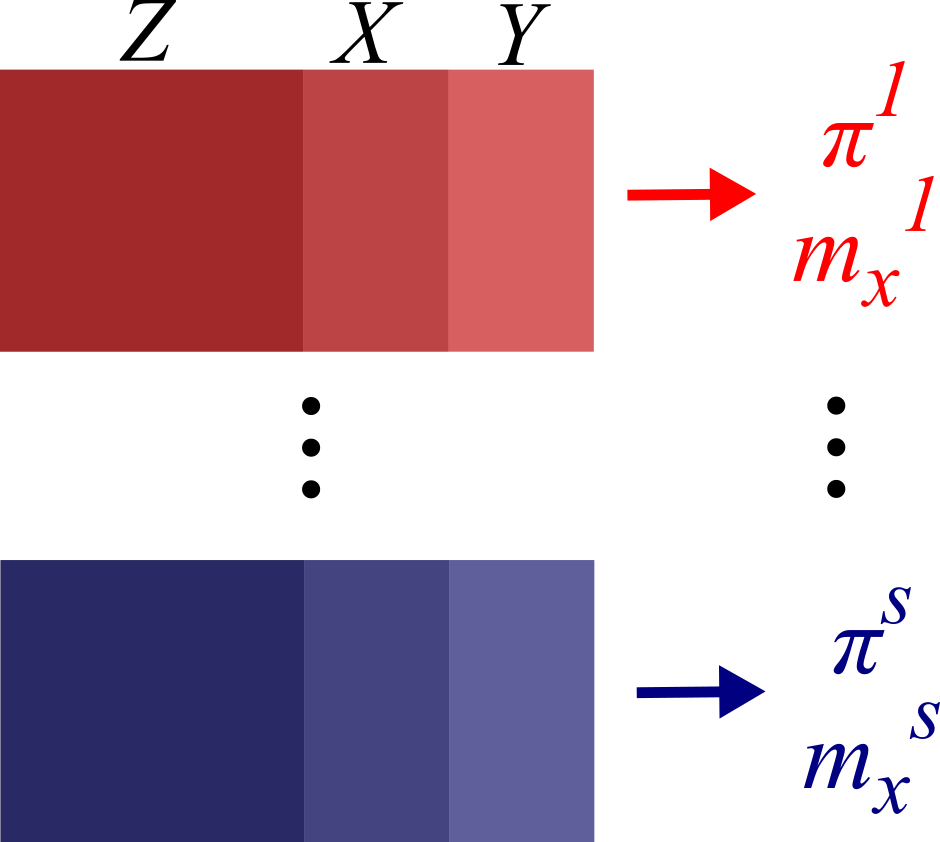
\includegraphics[scale=0.7]{images/step2_estimate.png}
\end{frame}

\begin{frame}{Step 3: Estimate $\psi^s$}
	\centering
	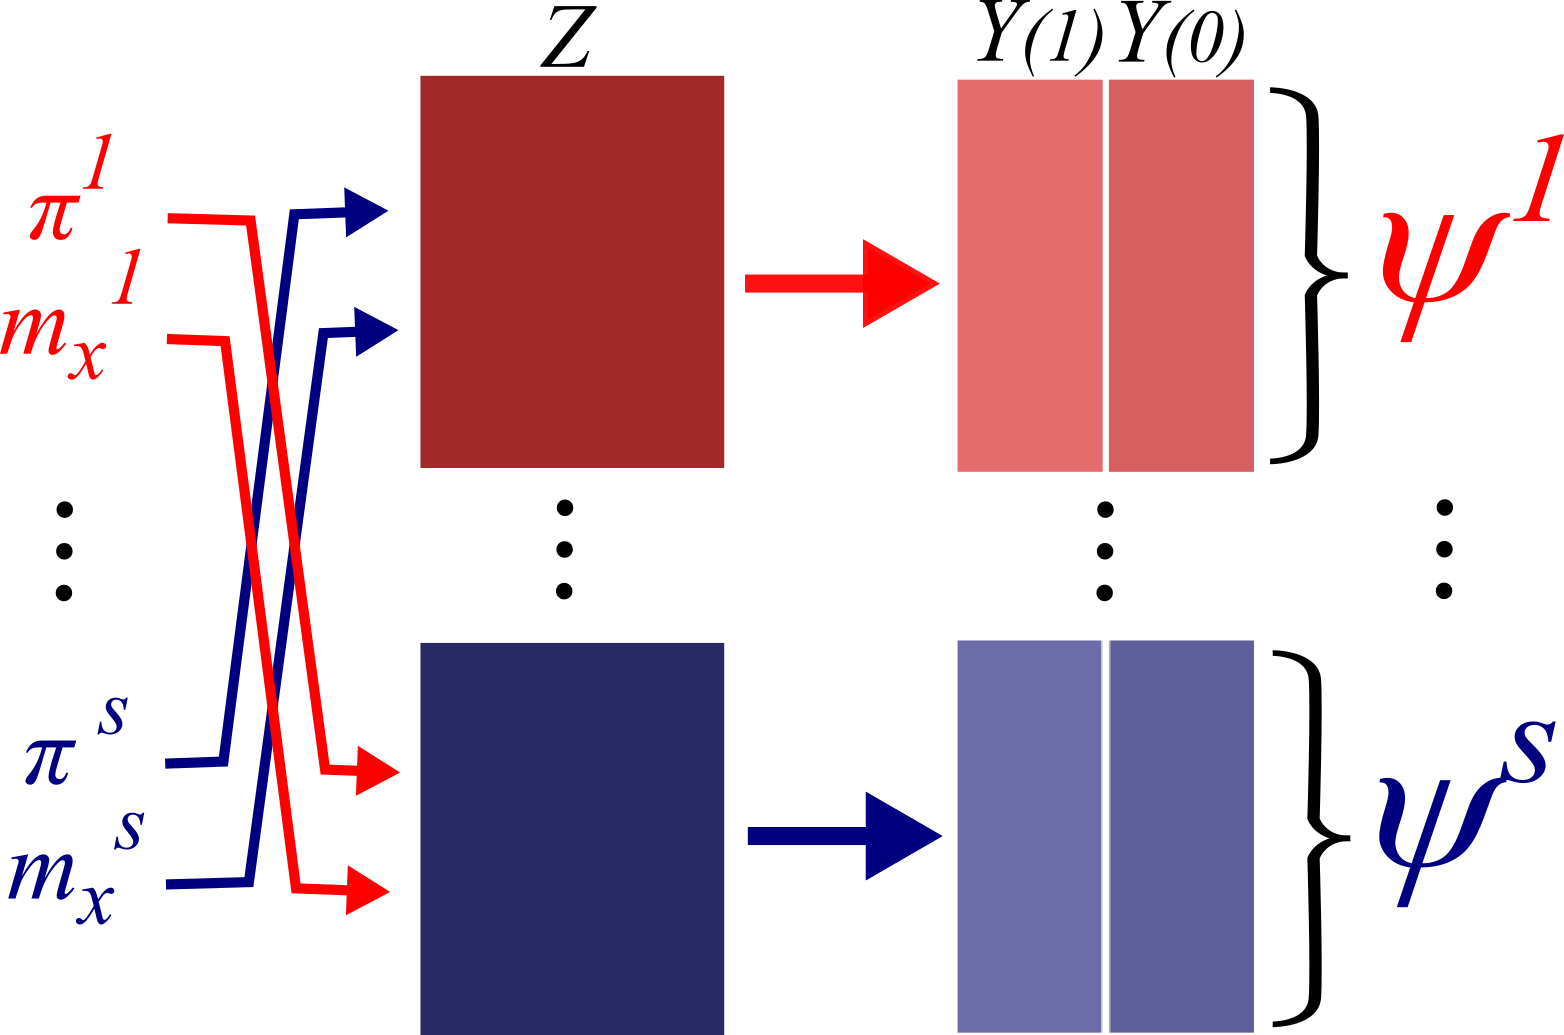
\includegraphics[scale=0.65]{images/step3_psi.png}
\end{frame}

\begin{frame}{Step 3: Estimate $\psi^s$}
	Augmented Inverse Probability Weighting
	\[\widehat{Y}^*_i(x) = \frac{I(X_i=x) Y_i}{\widehat{\pi}(Z_i)} + \frac{\widehat{m_x}(Z_i) (\widehat{\pi}(Z_i) - I(X_i=x))}{\widehat{\pi}(Z_i)}\]
	Then calculate
	\[\psi^s = \frac{1}{n_s} \sum_{i\in n_s} \widehat{Y}^*_i(x=1) - \widehat{Y}^*_i(x=0)\]
\end{frame}

%\begin{frame}{Step 3: Estimate $\psi^s$}
%	Targeted Maximum Likelihood Estimation
%	\[\widehat{Y}^*_i(x) = \text{expit}(\text{logit}(\widehat{m_x}(Z_i) + \widehat{\eta} \hat{H}(x,Z_i)))\]
%	where $\eta$ is estimated via
%	\[\text{logit}(Y_i) = \eta \hat{H}(X_i,Z_i) + \text{logit}(\widehat{m_{X_i}}(Z_i))\]
%	and 
%	\[\hat{H}(X_i,Z_i) = \frac{X_i}{\hat{\pi}(Z_i)} - \frac{1 - X_i}{1 - \hat{\pi}(Z_i)}\]
%\end{frame}

\begin{frame}{Step 4: Estimate $\psi^p$}
	Take the mean of all $\psi^s$
	\[\hat{\psi}^p = \frac{1}{s} \sum_{i=1}^{s} \hat{\psi}^s\]
\end{frame}

\begin{frame}{Step 5: Estimate $Var(\psi^p)$}
	Take the mean of all $Var(\psi^s)$
	\[\widehat{Var}(\hat{\psi}^p) = \frac{1}{s} \sum_{i=1}^{s} \widehat{Var}(\hat{\psi}^s)\]	
\end{frame}

\begin{frame}{Repeat for $p$ different partitions}
	Repeat previous steps for $p$ times\\~\\
	Summarize all different partitions used via
	\[\hat{\psi} = \text{median}(\hat{\psi}^p)\]
	\[\widehat{Var}(\hat{\psi}) = \text{median}\left(\widehat{Var}(\hat{\psi}^p) + (\hat{\psi} - \hat{\psi}^p)^2\right)\]
	\begin{itemize}
		\item Median rather than mean since more stable to outliers
	\end{itemize}
\end{frame}

\begin{frame}{Why $p$ Partitions?}
	Multiple splits
	\begin{itemize}
		\item Does not matter asymptotically
		\item For moderate $n$, $\hat{\psi}^p$ depends on the chosen split
		\begin{itemize}
			\item Increases \textit{statistical} efficiency
			\item Decreases \textit{computational} efficiency
		\end{itemize}
	\end{itemize}
	\begin{center}
		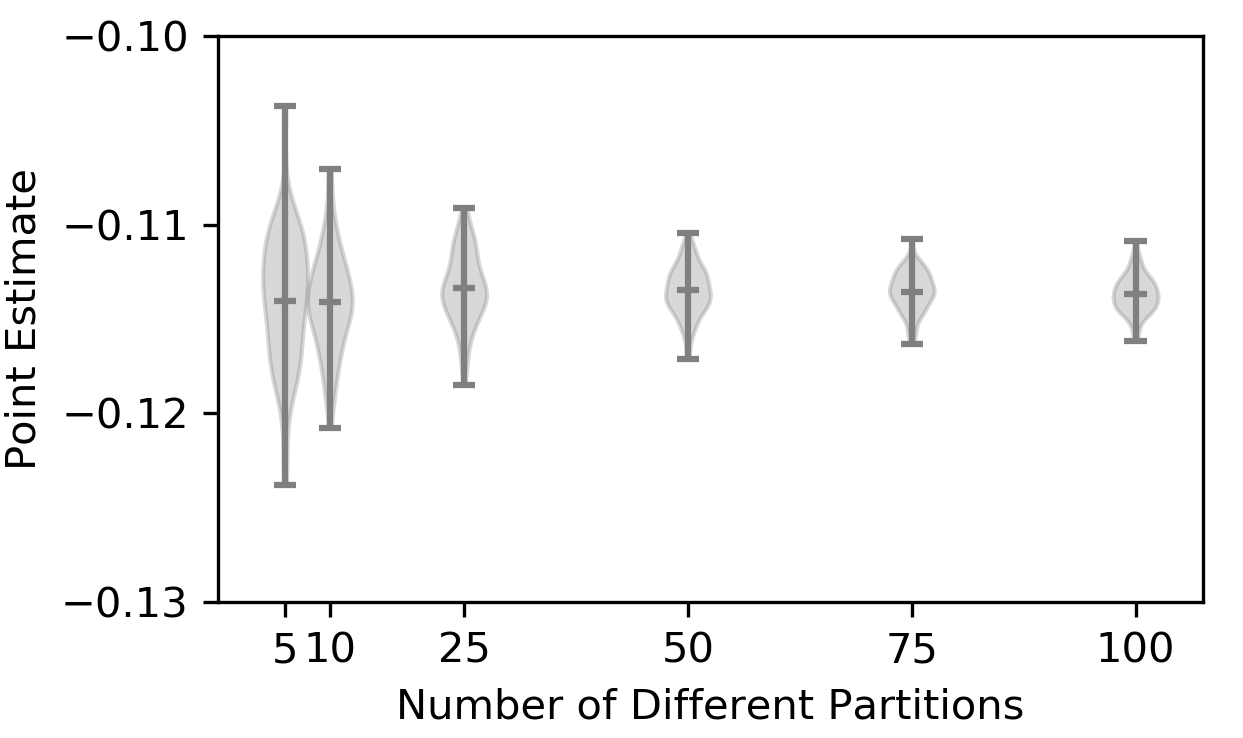
\includegraphics[scale=0.55]{images/multiple_p2.png}
	\end{center}
\end{frame}

\begin{frame}{Recommendations for Practical Application}
	\begin{enumerate}
		\item Flexible library of learners
		\begin{itemize}
			\item $k$-fold super-learner
			\item Variety of models
			\begin{itemize}
				\item Flexible regression, tree-based, gradient, etc.
			\end{itemize}
			\item Explore multiple tuning parameters
		\end{itemize}
		\item Doubly-robust estimator
		\item Cross-fitting
		\item Include transformations in data
	\end{enumerate}
\end{frame}

\begin{frame}{Software}
	Python
	\begin{itemize}
		\item \textit{zEpid}
		\begin{itemize}
			\item https://github.com/pzivich/zEpid
			\item v0.9.0+ Supports single and double cross-fit
			\item Support for both AIPW and TMLE
		\end{itemize}
		\item https://github.com/pzivich/publications-code
	\end{itemize}
	R
	\begin{itemize}
		\item https://github.com/yqzhong7/AIPW
		\item https://github.com/pzivich/publications-code
	\end{itemize}
\end{frame}

\section{Conclusions}

\begin{frame}{Conclusions}
	Machine learning is a useful tool for nuisance model specification
	\begin{itemize}
		\item Allow for flexible models
		\item Less concern over misspecification relative to parametric models
		\begin{itemize}
			\item Captures wider set of densities
		\end{itemize}
		\item Best benefit in my opinion
		\begin{itemize}
			\item Allows us to devote time to other biases
		\end{itemize}
	\end{itemize}
\end{frame}

\begin{frame}{~ }
	\centering
	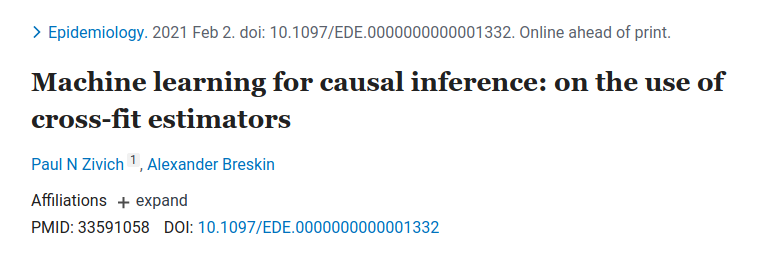
\includegraphics[scale=0.4]{images/paper_title.png}
\end{frame}

\begin{frame}{Further Reading}
	\scriptsize
	Doubly-robust estimators generally
	\begin{itemize}
		\item Daniel, Double Robustness, In: \textit{Statistics Reference Online} Wiley 2014
		\item Robins \& Ritov, Towards a Curse of Dimensionality Appropriate (CODA) Asymptotic Theory for Semi-Parametric Models, \textit{Statistics in Medicine} 1997
		\item Kennedy, Semiparametric theory and empirical processes in causal inference. In: \textit{Statistical Causal Inferences and their Applications in Public Health Research} Spring 2016 p141-167
	\end{itemize}
	Augmented inverse probability weighting
	\begin{itemize}
		\item Funk et al., Doubly Robust Estimation of Causal Effects. \textit{American Journal of Epidemiology} 2011, 173:7 p761-767
		\item Keil et al., Resolving an Apparent Paradox in Doubly Robust Estimators. \textit{American Journal of Epidemiology} 2018, 187:4 p891-892
		\item Bang \& Robins, Doubly Robust Estimation in Missing Data and Causal Inference Models. \textit{Biometrics} 2005, 61:4 p962-973
	\end{itemize}	
	Targeted maximum likelihood estimation
	\begin{itemize}
		\item Schuler \& Rose, Targeted Maximum Likelihood Estimation for Causal Inference in Observational Studies. \textit{American Journal of Epidemiology} 2017, 185:1 p65-67
	\end{itemize}		
\end{frame}

\begin{frame}{Further Reading}
	\scriptsize
	Machine Learning and Super learner 
	\begin{itemize}
		\item Bi et al., What is Machine Learning? A Primer for the Epidemiologist. \textit{American Journal of Epidemiology} Oct 2019, 188:12 p2222-2239
		\item Rose, Mortality Risk Score Prediction in an Elderly Population Using Machine Learning. \textit{American Journal of Epidemiology} 2013, 177:5 p443-452
		\item Naimi \& Balzer, Stacked Generalization: an Introduction to Super Learning. \textit{European Journal of Epidemiology} 2018, 33:5 p459-464
		\item Keil \& Edwards, You Are Smarter Than You Think: (Super) Machine Learning in Context. \textit{European Journal of Epidemiology} 2018, 33:5 p437-440		
	\end{itemize}
	Sample-splitting for machine learning
	\begin{itemize}
		\item Díaz, Machine learning in the estimation of causal effects: targeted minimum loss-based estimation and double/debiased machine learning, \textit{Biostatistics} April 2020, 21:2 p353–358
		\item Chernozhukov et al., Double/debiased machine learning for treatment and structural parameters, \textit{The Econometrics Journal} 2018 21, C1–C68
		\item Zheng \& van der Laan, Cross-validated targeted minimum-loss-based estimation. In: \textit{Targeted Learning} Springer 2011 p459–474
		\item Newey \& Robins, Cross-Fitting and Fast Remainder Rates for Semiparametric Estimation, \textit{arXiv}:1801.09138
	\end{itemize}
	Machine learning for causal inference
	\begin{itemize}
		\item Naimi et al., Challenges in Obtaining Valid Causal Effect Estimates with Machine Learning Algorithms. \textit{arXiv}:1711.07137
	\end{itemize}	
\end{frame}

\begin{frame}
	\frametitle{Acknowledgments}
	\faEnvelope \quad pzivich@live.unc.edu \qquad
	\faTwitter \quad @PausalZ \qquad
	\faGithub \quad pzivich\\
	\begin{center}
		{\footnotesize PNZ is supported by NICHD T32-HD091058}\\
	\end{center}
\end{frame}


\end{document}
